% hello.tex - Our first LaTeX example!

\documentclass{article}

\usepackage[top=1in, bottom=1in, left=0.5in, right=0.5in]{geometry} 
\usepackage{graphicx}
\usepackage{url}

\begin{document}



\title{Physics Behind the Simulation: A CS296 Report by Group 4}
\author{Pratik Fegade 120050004\\
\texttt{pratikf@cse.iitb.ac.in}\\
Krishna Deepak 120050057\\
\texttt{mskdeepak@cse.iitb.ac.in}\\
Bharath Kumar 120050058\\
\texttt{bharath@cse.iitb.ac.in}\\}
\date{\today}
\maketitle

\section{Introduction}
\hspace{1 cm}
The objective of the report is to make readers understand about the three extra parts that we added to the basic Box-2D animation. 
Also it is an exercise in understanding LaTeX \cite{lamport94} and BibTex \cite{bibtex_site} \cite{bibtex_wiki}. The assignment also provides an opportunity to know more about the Box2D physics engine. \cite{Box2d}

\section{Physics Behind Simulation}


%balls
\subsection{Balls on the Plank}
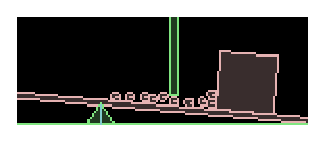
\includegraphics[width=7cm]{_-0}
\\*
\hspace{1 cm}
We have added 10 balls on the plank already present in the simulation. These balls have low masses and are perfectly elastic. The equations governing their colllisions are as follows.
\begin{equation}
	mu_x = mv_x
\end{equation}

\begin{equation}
	mu_y = - \epsilon mv_y
\end{equation}
where m is the mass (units: kg) of a ball, $u_x$ and $v_x$ are the initial and final velocities (units: $ms^{-1}$) of the ball in the x-direction. Similarly, $u_y$ and $v_y$ are the initial and final velocities (units: $ms^{-1}$) of the ball in the y-direction. The coefficient of restitution $\epsilon$ is 1 for the balls.



%block
\subsection{Block and its Supporting Plank}
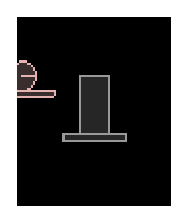
\includegraphics[width=5cm]{_-1}
\\*
\hspace{1 cm}
We have added a rectangular block that collides with the ball on its downward trajectory.
The impulse transferred by the falling ball on the plank is given by
\begin{equation}
 	J = m_b(v_b - u_b)
\end{equation}
where J is the angular impulse (units: $kg-m^2s^{-1}$), $m_b$ is the mass (units: kg) of the falling ball and $u_b$ and $v_b$ are the initial and final velocities (units: $ms^{-1}$) of the ball.
This angular impulse contributes to the rotation of the plank and the rotation and the translation of the block. This is described by the following equations
\begin{equation}
 	J = I_p \omega_p + m_{bl} v_{bl} + I_{bl} \omega_{bl}
\end{equation}
where $I_p$ and $I_{bl}$ are the moments of inertia (units: $kgm^2$) of the plank and the block, $\omega_p$ and $\omega_{bl}$ are the angular velocities (units: $rad^{-1}$) of the plank and the block, $v_{bl}$ is the velocity (units: $ms^{-1}$) of the block and $m_{bl}$ is the mass (units: kg) of the block. 


%vertical plank
\subsection{Rotating Vertical Plank}
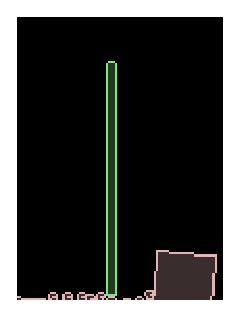
\includegraphics[width=5cm]{_-2}
\\*
\hspace{1 cm}
We have added a vertical plank, too.
\begin{equation}
	F_{bl} d_{centre} = I_p \omega_p
\end{equation}
where $I_p$ is the moment of inertia (units: $kgm^2$) of the plank, $\omega_p$ is the angular velocity (units: $rad^{-1}$) of the plank, $F_{bl}$ is the force (units: $kgms^{-2}$) applied by the block on the plank and $d_{centre}$ is the distance (units: m) of the point of collision from the centre of the plank. 

\section{Conclusions}
\hspace{1 cm}
The document thus talks about the additional components added to the provided simulation using Box2D. Specifically it describes the added objects and describes their physics to some extent.
 
\bibliographystyle{plain}
\bibliography{cs296_report_04.bib}

\end{document}
